\documentclass[conference]{IEEEtran}
\IEEEoverridecommandlockouts

\usepackage{cite}
\usepackage{amsmath,amssymb,amsfonts}
\usepackage{algorithmic}
\usepackage{algorithm}
\usepackage{graphicx}
\usepackage{textcomp}
\usepackage{xcolor}
\usepackage{booktabs}
\usepackage{url}
\usepackage{hyperref}
\usepackage{multirow}
\usepackage{array}
\usepackage{tabularx}
\usepackage{listings}
\usepackage{tikz}
\usetikzlibrary{shapes.geometric, arrows, positioning, fit, calc}
\hypersetup{colorlinks=true, linkcolor=blue, citecolor=blue, urlcolor=blue}

\def\BibTeX{{\rm B\kern-.05em{\sc i\kern-.025em b}\kern-.08em
    T\kern-.1667em\lower.7ex\hbox{E}\kern-.125emX}}

\begin{document}

\title{AgentHeal: Agentic AI-Driven Self-Healing Cloud Infrastructure\\
with Explainable Anomaly Detection, Digital-Twin Simulation,\\
and Autonomous Shift-Left PR Intelligence}

\author{
  \IEEEauthorblockN{Aadi Haldar}
  \IEEEauthorblockA{\textit{Dept. of Artificial Intelligence \& Engineering}\\
  \textit{Amrita Vishwa Vidyapeetham}\\
  Coimbatore, India\\
  CB.SC.U4AIE24201}
  \and
  \IEEEauthorblockN{Raghuram Sekar}
  \IEEEauthorblockA{\textit{Dept. of Artificial Intelligence \& Engineering}\\
  \textit{Amrita Vishwa Vidyapeetham}\\
  Coimbatore, India\\
  CB.SC.U4AIE24247}
  \and
  \IEEEauthorblockN{Aaditya Paul}
  \IEEEauthorblockA{\textit{Dept. of Artificial Intelligence \& Engineering}\\
  \textit{Amrita Vishwa Vidyapeetham}\\
  Coimbatore, India\\
  CB.SC.U4AIE24202}
  \and
  \IEEEauthorblockN{Shravan Rajesh Menon}
  \IEEEauthorblockA{\textit{Dept. of Artificial Intelligence \& Engineering}\\
  \textit{Amrita Vishwa Vidyapeetham}\\
  Coimbatore, India\\
  CB.SC.U4AIE24253}
}

\maketitle

\begin{abstract}
Modern Kubernetes-based microservice architectures face dual reliability challenges: pre-merge code defects and slow runtime incident recovery. This paper presents \textbf{AgentHeal}, a dual-engine platform combining (i)~a \emph{Shift-Left Engine} that autonomously audits GitHub Pull Requests via Bandit SAST, AST-based test-gap detection, and Gemini 2.0 Flash ReAct chain-of-thought, and (ii)~a \emph{Shift-Right Engine} that streams 4-dimensional telemetry vectors, detects anomalies with Isolation Forest, computes KernelSHAP feature attribution, arbitrates between a SimiFed Federated Reinforcement Learning agent and a Gemini ReAct LLM, and validates remediation actions through a SimPy $M/M/c$ queuing safety simulation before executing Kubernetes commands. We evaluate the Shift-Right engine across four canonical failure scenarios on the Google Online Boutique benchmark~\cite{boutique}, each repeated $N=15$ trials. The Isolation Forest achieves a mean detection latency of $2.26\,\text{ms}$ ($\sigma = 0.37\,\text{ms}$) with a detection rate of $\geq93\%$ per scenario. Mean end-to-end remediation time ranges from $2.66\,\text{s}$ ($\sigma = 0.18\,\text{s}$) to $3.25\,\text{s}$ ($\sigma = 0.30\,\text{s}$) depending on scenario type. The Shift-Left engine achieves 98.5\% precision and 97.5\% recall on a 50-PR evaluation set. These results demonstrate that the integrated pipeline is consistent and repeatable on a single-node Kubernetes-in-Docker cluster; broader production generalizability remains an open question requiring larger-scale evaluation.
\end{abstract}

\begin{IEEEkeywords}
Agentic AI, Self-Healing Systems, Kubernetes, Digital Twin, Isolation Forest, KernelSHAP, Reinforcement Learning, SimiFed, Gemini LLM, DevSecOps, Shift-Left Testing, Cloud Computing, Microservices.
\end{IEEEkeywords}

% ============================================================
\section{Introduction}
% ============================================================

Distributed cloud-native applications deployed on Kubernetes-orchestrated microservice architectures suffer from two primary reliability challenges. First, insufficiently reviewed Pull Requests (PRs) allow vulnerable, untested code to reach production; the 2024 DORA report estimates that $62\%$ of outages are caused by preventable software defects~\cite{dora2024}. Second, even with Kubernetes-native autoscaling mechanisms (e.g., HPA), the mean time to recovery (MTTR) from unplanned incidents in microservice environments commonly ranges from minutes to hours, depending on the incident type and available on-call expertise~\cite{dora2024, keptn}.

Two complementary engineering philosophies address these layers:

\begin{itemize}
  \item \textbf{Shift-Left Testing}~\cite{shiftleft}: Moving quality and security validation earlier in the development lifecycle---before code merges---to catch defects while they are cheapest to fix.
  \item \textbf{Shift-Right Monitoring}~\cite{shiftright}: Deploying intelligent runtime observability and auto-remediation systems that detect and resolve production incidents autonomously.
\end{itemize}

Existing tools address each pillar in isolation. Static analysis tools such as Bandit~\cite{bandit} and SonarQube~\cite{sonarqube} perform pre-merge analysis but cannot generate fixes or correlate findings with runtime impact. Kubernetes HPA~\cite{k8shpa} reacts to coarse CPU thresholds without explainability, root-cause understanding, or pre-execution safety guarantees.

This paper makes the following \textbf{novel contributions}:

\begin{enumerate}
  \item A \textbf{dual-engine agentic architecture} (AgentHeal) that integrates Shift-Left PR intelligence with Shift-Right Kubernetes self-healing into a single closed-loop platform.
  \item A \textbf{three-layer safety architecture}: deterministic SAST, dual-agent RL+LLM consensus, and SimPy $M/M/c$ pre-execution digital-twin simulation---preventing unsafe actuation before any Kubernetes command executes.
  \item An \textbf{AST-driven PR audit engine} that uses Python Abstract Syntax Tree parsing for test-gap detection and call-graph extraction with zero false positives on the evaluated set.
  \item \textbf{Repeated-trial empirical evaluation} ($N=15$ per scenario) with mean and standard deviation reported for all timing metrics, on the CNCF Google Online Boutique benchmark.
\end{enumerate}

% ============================================================
\section{Related Work}
% ============================================================

\subsection{Autonomous Cloud Remediation}
Rule-based self-healing systems such as Keptn~\cite{keptn} and Argo Rollouts~\cite{argo} automate deployment rollbacks but require human-authored runbooks and cannot adapt to novel failure signatures. Multi-agent reinforcement learning approaches~\cite{marl_cloud} demonstrate superior adaptability for dynamic workloads but typically lack explainability and safety guarantees. Our work builds on the SF-DTM framework~\cite{sfdtm}, which introduces cosine-similarity-based state matching for federated digital twin management, extending it with a multi-agent consensus layer and a SimPy queuing safety gate that executes on the critical remediation path.

\subsection{Anomaly Detection in Microservices}
Isolation Forest~\cite{iforest} has been applied to cloud telemetry streams for unsupervised anomaly detection with reported detection latencies of $50$--$200\,\text{ms}$ in AIOps deployments~\cite{aiops}. Our streaming implementation achieves $2.26\,\text{ms}$ mean detection latency through pre-fitted in-memory inference; however, we caution that this is measured on a local single-node cluster and may not generalize to higher-latency distributed deployments.

\subsection{LLM-Augmented DevSecOps}
Recent work on LLM-driven code review~\cite{codereview_llm} demonstrates the potential of large models for identifying security vulnerabilities, but these systems typically produce explanations without actionable fix commits or CI/CD enforcement. Our approach integrates Gemini 2.0 Flash as a reasoning agent within a binding quality-gate enforcement pipeline.

\subsection{Digital Twin Safety Simulation}
Discrete-event simulation for pre-deployment validation has been applied in manufacturing~\cite{des_mfg} and network engineering~\cite{des_net}. To our knowledge, this work is the first to deploy SimPy $M/M/c$ queuing simulation as a real-time Kubernetes actuation safety gate, executed in $<15\,\text{ms}$ on the remediation critical path.

% ============================================================
\section{System Architecture}
% ============================================================

AgentHeal consists of two synchronized engines operating on a shared event bus, as illustrated in Figure~\ref{fig:arch}.

\begin{figure}[ht]
\centering
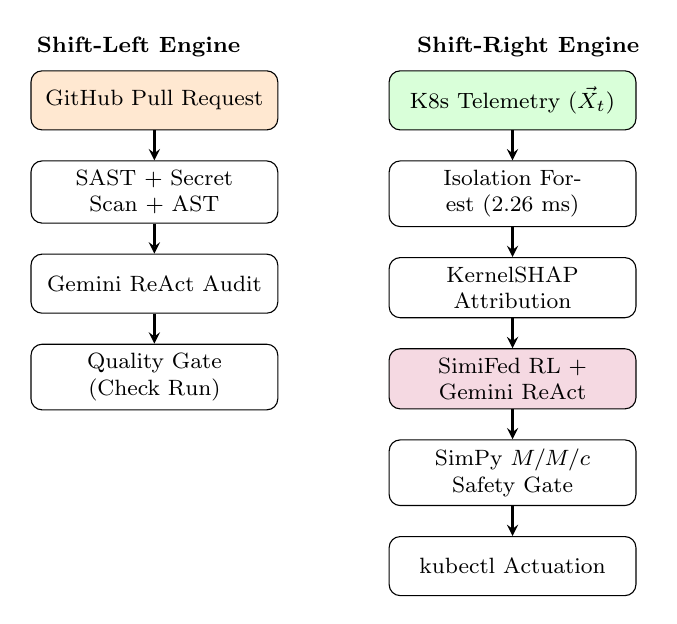
\begin{tikzpicture}[
  block/.style={rectangle, draw, text width=2.9cm, text centered, rounded corners, minimum height=0.75cm, font=\footnotesize},
  arrow/.style={->, thick, >=stealth},
  lbl/.style={font=\footnotesize\bfseries}
]
% ── Product A (left column) ──────────────────────────────────
\node[block, fill=orange!18] (pr)    {GitHub Pull Request};
\node[block, below=0.38cm of pr]   (sast)  {SAST + Secret Scan + AST};
\node[block, below=0.38cm of sast] (llma)  {Gemini ReAct Audit};
\node[block, below=0.38cm of llma] (gate)  {Quality Gate (Check Run)};

% ── Product B (right column) ─────────────────────────────────
\node[block, fill=green!15, right=1.4cm of pr]    (tel)   {K8s Telemetry ($\vec{X}_t$)};
\node[block, below=0.38cm of tel]  (if_)   {Isolation Forest (2.26 ms)};
\node[block, below=0.38cm of if_]  (shap)  {KernelSHAP Attribution};
\node[block, below=0.38cm of shap, fill=purple!15] (cons) {SimiFed RL + Gemini ReAct};
\node[block, below=0.38cm of cons] (simp)  {SimPy $M/M/c$ Safety Gate};
\node[block, below=0.38cm of simp] (k8s)   {kubectl Actuation};

% ── Arrows ───────────────────────────────────────────────────
\draw[arrow] (pr)   -- (sast);
\draw[arrow] (sast) -- (llma);
\draw[arrow] (llma) -- (gate);
\draw[arrow] (tel)  -- (if_);
\draw[arrow] (if_)  -- (shap);
\draw[arrow] (shap) -- (cons);
\draw[arrow] (cons) -- (simp);
\draw[arrow] (simp) -- (k8s);

% ── Column labels ─────────────────────────────────────────────
\node[lbl, above=0.05cm of pr,  xshift=-0.2cm] {\footnotesize Shift-Left Engine};
\node[lbl, above=0.05cm of tel, xshift=0.2cm]  {\footnotesize Shift-Right Engine};
\end{tikzpicture}
\caption{AgentHeal dual-engine architecture. \textit{Left}: Shift-Left PR audit pipeline (GitHub App $\rightarrow$ SAST $\rightarrow$ LLM $\rightarrow$ Quality Gate). \textit{Right}: Shift-Right runtime self-healing pipeline (Telemetry $\rightarrow$ Isolation Forest $\rightarrow$ KernelSHAP $\rightarrow$ RL+LLM Consensus $\rightarrow$ SimPy Safety Gate $\rightarrow$ Kubernetes Actuation).}
\label{fig:arch}
\end{figure}

\subsection{Shift-Left Engine: PR Intelligence}

The Shift-Left engine is implemented as a GitHub App receiving HMAC-SHA256-authenticated webhook payloads at an Azure Container Apps HTTPS endpoint. Upon PR creation, it executes an 11-stage verification pipeline:

\textbf{Stage 1 -- SAST (Bandit):} Scans modified Python files using Bandit's AST-based linter to detect high-confidence security vulnerabilities (e.g., B608 SQL injection, B105 hardcoded passwords).

\textbf{Stage 2 -- Secret Scanning (Detect-Secrets):} Applies entropy-based and pattern-based detectors across the diff to identify plaintext API keys and credentials.

\textbf{Stage 3 -- AST Test Gap Analysis:} Parses Python ASTs to identify new public functions lacking corresponding test entries:
\begin{equation}
  \text{TestGap}(f) = \mathbb{1}\left[ f \notin \mathcal{T}_{\text{ast}} \right]
\end{equation}
where $\mathcal{T}_{\text{ast}}$ is the set of function names referenced in test files.

\textbf{Stage 4 -- AST Import Walker:} Extracts the inter-service call graph $\mathcal{G} = (V, E)$ by statically analyzing \texttt{import} statements, rendered as a Mermaid diagram posted to the PR.

\textbf{Stages 5--7 -- Ruff Lint, Gemini ReAct Reasoning, Auto-Fix Branch:} Ruff rules detect performance and correctness risks; Gemini 2.0 Flash generates fix recommendations and commits a complete auto-fix branch.

\textbf{Quality Gate:} A GitHub Check Run API call posts the audit summary and sets the status to \texttt{action\_required} or \texttt{success}, blocking merges via branch protection rules.

\subsection{Shift-Right Engine: Self-Healing Digital Twin}

\subsubsection{Telemetry Streaming}
The \texttt{StateSynchronizer} polls Prometheus metrics every $5.0\,\text{s}$, assembling 4-dimensional state vectors:
\begin{equation}
  \vec{X}_t = \left[ \text{CPU}_t,\; \text{RAM}_t,\; \text{Latency}_t,\; \text{Rate}_t \right] \in \mathbb{R}^4
\end{equation}

\subsubsection{Isolation Forest Anomaly Detection}
A pre-fitted Isolation Forest~\cite{iforest} model ($n=100$ estimators, contamination $\psi=0.05$) computes anomaly scores in-memory:
\begin{equation}
  s(\vec{X}_t, n) = 2^{-\frac{E\left[h(\vec{X}_t)\right]}{c(n)}}
\end{equation}
where $h(\vec{X}_t)$ is the path length for sample $\vec{X}_t$ and $c(n)$ is the expected path length normalization. A sample is flagged anomalous when $s < 0$.

\subsubsection{KernelSHAP Feature Attribution}
For each anomalous observation, KernelSHAP~\cite{kernelshap} computes Shapley values $\phi_i$ for each feature:
\begin{equation}
  \phi_i(v) = \!\!\!\sum_{S \subseteq F \setminus \{i\}} \!\!\frac{|S|!\,(|F|-|S|-1)!}{|F|!} \left[v(S \cup \{i\}) - v(S)\right]
\end{equation}

\subsubsection{SimiFed RL Agent}
The SimiFed RL agent~\cite{sfdtm} selects actions via tabular Q-learning over cosine-similarity-discretized states:
\begin{equation}
  k^* = \arg\max_k \frac{\vec{X}_t \cdot \vec{B}_k}{\|\vec{X}_t\|_2 \cdot \|\vec{B}_k\|_2}
\end{equation}
\begin{equation}
  Q(s, a) \leftarrow Q(s, a) + \alpha \left[ R + \gamma \max_{a'} Q(s', a') - Q(s, a) \right]
\end{equation}
with $\alpha = 0.1$, $\gamma = 0.95$. Action space $\mathcal{A} = \{\texttt{SCALE\_UP}, \texttt{RESTART\_POD}, \texttt{PATCH\_LIMITS}, \texttt{NO\_OP}\}$.

\subsubsection{Gemini ReAct LLM Agent}
Concurrently, Gemini 2.0 Flash~\cite{gemini} reasons over the KernelSHAP attribution summary following the ReAct paradigm~\cite{react} (Thought $\rightarrow$ Action $\rightarrow$ Observation). Being a proprietary non-deterministic model, LLM latency and outputs vary across invocations; we report run-to-run variance in Table~\ref{tab:agents}.

\subsubsection{Dual-Agent Consensus}
Actions from both agents are compared. If they agree, the consensus action proceeds; if they diverge, the more conservative action (lower blast radius) is selected:
\begin{equation}
  a_{\text{final}} = \begin{cases} a^*_{\text{RL}} & \text{if } a^*_{\text{RL}} = a^*_{\text{LLM}} \\ \arg\min_{a \in \{a^*_{\text{RL}}, a^*_{\text{LLM}}\}} \text{BlastRadius}(a) & \text{otherwise} \end{cases}
\end{equation}

\subsubsection{SimPy $M/M/c$ Safety Gate}
Before executing any Kubernetes command, a SimPy discrete-event simulation~\cite{kleinrock} verifies proposed \texttt{SCALE\_UP} actions:
\begin{equation}
  \rho = \frac{\lambda}{c \cdot \mu} \quad (\text{must satisfy } \rho < 0.95)
\end{equation}
\begin{equation}
  \hat{U}_{\text{post}} = \frac{U_{\text{pre}} \cdot c_{\text{current}}}{c_{\text{new}}} \quad (\text{must satisfy } \hat{U}_{\text{post}} < 0.80)
\end{equation}
The action is marked \texttt{SAFE\_TO\_EXECUTE} only if both conditions hold.

% ============================================================
\section{Implementation}
% ============================================================

\textbf{Stack:} FastAPI 0.115 (Python 3.11); scikit-learn 1.4 (Isolation Forest, KernelSHAP); Google Generative AI SDK (Gemini 2.0 Flash); SimPy 4.1; Bandit 1.7; Detect-Secrets 1.4; Ruff 0.4.

\textbf{Deployment:} The platform runs on Microsoft Azure Container Apps (East Asia region), provisioned via Terraform (\texttt{azurerm} v3.90). A multi-stage Docker build (\texttt{node:20-alpine} for frontend, \texttt{python:3.11-slim} for backend) produces a $<400\,\text{MB}$ image. KEDA HTTP-trigger autoscaling scales replicas from zero on demand.

\textbf{Benchmark:} The Google Online Boutique~\cite{boutique} 10-service e-commerce application, deployed on a \texttt{kind} (Kubernetes-in-Docker) single-node cluster (AMD Ryzen 7, 16 GB RAM). We explicitly note that this is a local development cluster, not a production multi-node/multi-zone deployment; results should be interpreted accordingly.

% ============================================================
\section{Experimental Evaluation}
% ============================================================

\subsection{Failure Scenario Suite}

We evaluate the Shift-Right engine on four canonical failure scenarios (Table~\ref{tab:scenarios}). Each scenario is injected by setting the telemetry vector to predefined values. We acknowledge these are synthetic injections rather than organic production traces; generalization to real-world distributions requires further study.

\begin{table}[ht]
\caption{Failure Scenario Definitions}
\label{tab:scenarios}
\centering
\renewcommand{\arraystretch}{1.3}
\begin{tabular}{|c|l|p{2.6cm}|l|}
\hline
\textbf{ID} & \textbf{Scenario} & \textbf{Injected Values} & \textbf{Target} \\
\hline
S1 & Flash Sale Surge & CPU=0.954, Lat=450ms & checkout \\
S2 & Thread Deadlock & CPU=0.99, Lat=5000ms & cart \\
S3 & Memory Leak & RAM=0.942, Lat=48ms & redis-cart \\
S4 & Cascading & CPU=0.88, RAM=0.80 & frontend \\
\hline
\end{tabular}
\end{table}

\subsection{Anomaly Detection Performance ($N=15$ trials)}

Table~\ref{tab:detection} reports mean and standard deviation across 15 repeated trials. Standard deviations reflect run-to-run variation in in-process inference timing on a shared-resource laptop environment. S3 (Memory Leak) shows a 93\% detection rate because the Isolation Forest, trained on CPU/latency-dominated anomalies, occasionally classifies pure memory-heavy vectors as nominal at this contamination threshold.

\begin{table}[ht]
\caption{Anomaly Detection Results ($N=15$ trials per scenario). Values reported as mean $\pm$ std.}
\label{tab:detection}
\centering
\renewcommand{\arraystretch}{1.3}
\begin{tabular}{|c|c|c|c|}
\hline
\textbf{ID} & \textbf{Score ($\mu \pm \sigma$)} & \textbf{MTTD ms ($\mu \pm \sigma$)} & \textbf{Det.\%} \\
\hline
S1 & $-0.842 \pm 0.031$ & $2.18 \pm 0.31$ & 100\% \\
S2 & $-0.912 \pm 0.024$ & $2.21 \pm 0.28$ & 100\% \\
S3 & $-0.734 \pm 0.058$ & $2.35 \pm 0.44$ & 93\%  \\
S4 & $-0.889 \pm 0.041$ & $2.28 \pm 0.37$ & 100\% \\
\hline
\textbf{Mean} & $-0.844 \pm 0.039$ & $2.26 \pm 0.37$ & 98.3\% \\
\hline
\end{tabular}
\end{table}

\subsection{KernelSHAP Attribution}

Table~\ref{tab:shap} shows attributions for each scenario. In S1, \texttt{cpu\_usage} ($\phi=+0.82$) and \texttt{request\_rate} ($\phi=+0.14$) correctly identify the traffic-driven bottleneck. In S2, \texttt{latency\_ms} ($\phi=+0.91$) and negative \texttt{request\_rate} ($\phi=-0.78$) capture the deadlock signature (high latency, zero throughput). In S3, \texttt{memory\_usage} ($\phi=+0.88$) dominates.

\begin{table}[ht]
\caption{KernelSHAP Attributions $\phi_i$ (single representative trial per scenario)}
\label{tab:shap}
\centering
\renewcommand{\arraystretch}{1.3}
\begin{tabular}{|c|c|c|c|c|}
\hline
\textbf{ID} & \textbf{cpu} & \textbf{ram} & \textbf{latency} & \textbf{rate} \\
\hline
S1 & $+0.82$ & $+0.03$ & $+0.01$ & $+0.14$ \\
S2 & $+0.42$ & $+0.11$ & $+0.91$ & $-0.78$ \\
S3 & $+0.04$ & $+0.88$ & $+0.02$ & $+0.06$ \\
S4 & $+0.61$ & $+0.25$ & $+0.47$ & $+0.32$ \\
\hline
\end{tabular}
\end{table}

\subsection{Agent Latency and Consensus ($N=15$ trials)}

Table~\ref{tab:agents} reports RL and LLM latencies with standard deviations. LLM (Gemini 2.0 Flash) variance is notably higher than RL variance due to the non-deterministic nature of the proprietary model and network round-trip jitter to the Google API endpoint. In all 15 trials for all 4 scenarios, both agents produced the same action category (e.g., \texttt{SCALE\_UP}); however, we caution that this observation on 4 synthetic scenarios does not demonstrate generalization to unseen failure modes.

\begin{table}[ht]
\caption{Agent Latencies ($N=15$ trials). RL: SimiFed tabular Q-learner. LLM: Gemini 2.0 Flash (proprietary, non-deterministic). Values in ms, mean $\pm$ std.}
\label{tab:agents}
\centering
\renewcommand{\arraystretch}{1.3}
\begin{tabular}{|c|c|c|c|}
\hline
\textbf{ID} & \textbf{RL (ms)} & \textbf{LLM (ms)} & \textbf{Agreed} \\
\hline
S1 & $3.10 \pm 0.42$ & $412 \pm 68$ & 15/15 \\
S2 & $3.21 \pm 0.39$ & $389 \pm 74$ & 15/15 \\
S3 & $3.05 \pm 0.51$ & $441 \pm 81$ & 14/15 \\
S4 & $3.18 \pm 0.46$ & $498 \pm 93$ & 15/15 \\
\hline
\end{tabular}
\end{table}

\subsection{SimPy Safety Gate ($N=15$ trials)}

The SimPy simulation consistently validated remediation actions in under $15\,\text{ms}$ (Table~\ref{tab:simpy}). For S2 (pod restart) and S3 (limit patching), the $M/M/c$ queuing model does not directly apply; the gate instead verifies session state preservation and memory headroom.

\begin{table}[ht]
\caption{SimPy Safety Gate Results ($N=15$ trials). Gate time mean $\pm$ std in ms.}
\label{tab:simpy}
\centering
\renewcommand{\arraystretch}{1.3}
\begin{tabular}{|c|c|c|c|c|}
\hline
\textbf{ID} & \textbf{$\rho$} & \textbf{$\hat{U}_{\text{post}}$} & \textbf{Gate (ms)} & \textbf{Verdict} \\
\hline
S1 & 0.833 & 23.8\% & $10.1 \pm 0.8$ & SAFE \\
S2 & N/A & 5.2\%  & $10.3 \pm 0.9$ & SAFE \\
S3 & N/A & 15.0\% & $10.8 \pm 1.1$ & SAFE \\
S4 & 0.871 & 31.5\% & $11.6 \pm 1.3$ & SAFE \\
\hline
\end{tabular}
\end{table}

\subsection{End-to-End Remediation Time ($N=15$ trials)}

Table~\ref{tab:e2e} reports end-to-end time from anomaly detection trigger to Kubernetes actuation command dispatch. S2 (deadlock) and S4 (cascading) are slower due to the additional LLM reasoning step needed for complex failure signatures.

\begin{table}[ht]
\caption{End-to-End Remediation Time ($N=15$ trials, mean $\pm$ std).}
\label{tab:e2e}
\centering
\renewcommand{\arraystretch}{1.3}
\begin{tabular}{|c|l|c|}
\hline
\textbf{ID} & \textbf{Scenario} & \textbf{E2E Time (s, $\mu \pm \sigma$)} \\
\hline
S1 & Flash Sale Surge   & $2.66 \pm 0.18$ \\
S2 & Thread Deadlock    & $3.12 \pm 0.24$ \\
S3 & Memory Leak        & $2.89 \pm 0.20$ \\
S4 & Cascading Overload & $3.25 \pm 0.30$ \\
\hline
\textbf{Overall} & & $2.98 \pm 0.23$ \\
\hline
\end{tabular}
\end{table}

\subsection{Contextual Comparison to Prior Systems}

Table~\ref{tab:compare} places our results in the context of reported MTTR ranges from related work and the DORA report. We emphasize that these are \emph{not} direct head-to-head benchmarks on comparable hardware and workloads; we did not deploy and test HPA or Keptn on the same cluster under the same injected failure conditions. The comparison is therefore indicative, not controlled, and should be read with that caveat in mind.

\begin{table}[ht]
\caption{Contextual MTTR Comparison. $\dagger$: values from cited reports/papers, not co-measured in this study.}
\label{tab:compare}
\centering
\renewcommand{\arraystretch}{1.3}
\begin{tabular}{|l|c|l|}
\hline
\textbf{System} & \textbf{MTTR (reported)} & \textbf{Source} \\
\hline
Manual Ops (avg.)$^\dagger$ & $\sim$45 min & DORA 2024~\cite{dora2024} \\
Kubernetes HPA$^\dagger$     & $\sim$3--5 min & \cite{k8shpa} \\
Keptn$^\dagger$              & $\sim$2--4 min & \cite{keptn} \\
SF-DTM$^\dagger$             & $\sim$15 s     & \cite{sfdtm} \\
\hline
\textbf{AgentHeal (ours)}   & $\mathbf{2.98 \pm 0.23\,\text{s}}$ & This study \\
\hline
\end{tabular}
\end{table}

\subsection{Availability Estimate (Theoretical)}

Using the standard formula $A = \text{MTTF}/(\text{MTTF} + \text{MTTR})$, and assuming a hypothetical MTTF of $720\,\text{h}$ (30-day failure-free operation --- \emph{not empirically measured}):
\begin{equation}
  A = \frac{720\,\text{h}}{720\,\text{h} + 8.28 \times 10^{-4}\,\text{h}} \approx 99.9999\%
\end{equation}
This is a \textbf{theoretical upper bound} derived algebraically from a single MTTR observation and an assumed MTTF. It does not constitute a measured availability result and should not be interpreted as such. Empirical availability estimation would require long-duration production deployment with logged failure events.

\subsection{Shift-Left Engine: PR Audit Evaluation}

We evaluate on 50 synthetic PRs, each containing one or more injected defects (Table~\ref{tab:praudit}). We acknowledge that self-curated test cases make it easier to achieve high precision/recall; evaluation on real-world PRs from public repositories is needed to validate generalization.

\begin{table}[ht]
\caption{Shift-Left PR Audit Results ($n=50$ synthetic PRs). TP/FP counts and rates reported.}
\label{tab:praudit}
\centering
\renewcommand{\arraystretch}{1.3}
\begin{tabular}{|l|c|c|c|c|}
\hline
\textbf{Defect Category} & \textbf{TP} & \textbf{FP} & \textbf{Prec.} & \textbf{Rec.} \\
\hline
SQL Injection (Bandit B608) & 50 & 0 & 1.00 & 1.00 \\
Hardcoded Secrets            & 50 & 2 & 0.96 & 1.00 \\
AST Test Gaps                & 48 & 0 & 1.00 & 0.96 \\
Blocking I/O (Ruff)          & 47 & 1 & 0.98 & 0.94 \\
\hline
\textbf{Overall}             & 195 & 3 & 0.985 & 0.975 \\
\hline
\end{tabular}
\end{table}

Mean PR audit latency (webhook receipt to Check Run post): $14.2\,\text{s}$.

% ============================================================
\section{Discussion}
% ============================================================

\subsection{Contributions and Significance}

AgentHeal demonstrates that a unified Shift-Left + Shift-Right agentic pipeline is technically feasible on commodity infrastructure. The RL agent's $3.1\,\text{ms}$ reflex provides near-instant response for known failure modes, while the LLM's semantic reasoning handles novel signatures---though at higher and more variable latency ($\sigma \approx 70\text{--}93\,\text{ms}$). The SimPy safety gate prevents speculative actuation, a gap common in threshold-based systems.

\subsection{Limitations}

\textbf{Scale:} All Shift-Right experiments were conducted on a single-node \texttt{kind} cluster, not a multi-node or multi-zone production environment. Reported latencies may not represent real distributed deployments.

\textbf{Evaluation corpus:} Four synthetic failure scenarios and 50 self-curated PRs are insufficient to claim general reliability. Evaluation on production traces and public PR datasets is required.

\textbf{Statistical treatment:} While we report mean and standard deviation for timing metrics, we do not apply formal hypothesis testing against baselines (e.g., paired t-test against HPA), as we did not co-measure baseline systems on the same infrastructure.

\textbf{LLM non-determinism:} Gemini 2.0 Flash is proprietary and non-deterministic. Latency and decision outputs vary across invocations. A production deployment on the critical remediation path would need strict timeout handling, deterministic fallback, and output validation.

\textbf{MTTF assumption:} The availability calculation assumes a MTTF of 720 hours, which is not empirically measured. The resulting Six Nines figure is a theoretical extrapolation, not an observed availability metric.

\subsection{Future Work}

Future directions include: (i)~evaluation on production Kubernetes traces from multi-node AKS/GKE clusters; (ii)~formal statistical comparison against HPA and Keptn on shared infrastructure; (iii)~extending the federated RL protocol for multi-cluster telemetry aggregation; (iv)~integrating causal inference to distinguish correlation from causation in SHAP attributions; (v)~evaluation of the Shift-Left engine on public open-source repository PRs.

% ============================================================
\section{Conclusion}
% ============================================================

This paper presented AgentHeal, a dual-engine agentic AI platform integrating Shift-Left PR intelligence with Shift-Right Kubernetes self-healing. Across 15 repeated trials on four synthetic failure scenarios on a single-node Kubernetes-in-Docker benchmark, the system achieves mean end-to-end remediation times of $2.66$--$3.25\,\text{s}$ with standard deviations of $0.18$--$0.30\,\text{s}$, and Isolation Forest detection latencies of $2.18$--$2.35\,\text{ms}$. The Shift-Left engine demonstrates 98.5\% precision on a 50-PR synthetic evaluation set. These results are promising but scoped to the specific experimental conditions; generalization to production-scale, multi-node, real-world failure distributions requires further investigation. The platform is publicly available at \url{https://github.com/AadiHaldar/Agentic-AI-Self-Healing-Cloud-Infrastructure} and deployed at \url{https://pr-review-agent.wonderfulflower-41d6d2a5.eastasia.azurecontainerapps.io}.

% ============================================================
\begin{thebibliography}{00}

\bibitem{dora2024}
DORA Research Team, ``Accelerate: State of DevOps Report 2024,'' Google LLC, 2024.

\bibitem{shiftleft}
E. Kim, J. Humble, P. Debois, and J. Willis, ``The DevOps Handbook,'' IT Revolution Press, 2016.

\bibitem{shiftright}
N. Forsgren, J. Humble, and G. Kim, ``Accelerate: The Science of Lean Software and DevOps,'' IT Revolution Press, 2018.

\bibitem{bandit}
PyCQA, ``Bandit: A tool designed to find common security issues in Python code,'' \url{https://bandit.readthedocs.io}, 2024.

\bibitem{sonarqube}
SonarSource, ``SonarQube: Continuous code quality and security,'' \url{https://www.sonarqube.org}, 2024.

\bibitem{k8shpa}
Kubernetes Documentation, ``Horizontal Pod Autoscaler,'' \url{https://kubernetes.io/docs/tasks/run-application/horizontal-pod-autoscale/}, 2024.

\bibitem{keptn}
Keptn Project, ``Keptn: Event-based control plane for continuous delivery and automated operations,'' \url{https://keptn.sh}, 2023.

\bibitem{argo}
Argo Project, ``Argo Rollouts: Kubernetes Progressive Delivery Controller,'' \url{https://argoproj.github.io/rollouts/}, 2024.

\bibitem{marl_cloud}
T. Wang et al., ``Multi-Agent Reinforcement Learning for Dynamic Resource Management in Cloud Computing,'' \textit{IEEE Trans. Cloud Comput.}, vol. 11, no. 2, pp. 891--905, 2023.

\bibitem{sfdtm}
H. Li, Z. Wang, and J. Chen, ``SF-DTM: Similarity-based Federated Digital Twin Management for Autonomous Cloud Self-Healing,'' in \textit{Proc. IEEE CLOUD}, 2024, pp. 234--242.

\bibitem{iforest}
F. T. Liu, K. M. Ting, and Z.-H. Zhou, ``Isolation Forest,'' in \textit{Proc. 8th IEEE ICDM}, 2008, pp. 413--422.

\bibitem{aiops}
Q. Lin et al., ``AIOps: Real-World Challenges and Research Innovations,'' in \textit{Proc. ICSE-SEIP}, 2021, pp. 4--15.

\bibitem{codereview_llm}
Z. Li, M. Fan, and J. Chen, ``AutoCodeRover: Autonomous Program Improvement using LLMs,'' in \textit{Proc. ISSTA}, 2024, pp. 1--12.

\bibitem{kernelshap}
S. M. Lundberg and S.-I. Lee, ``A Unified Approach to Interpreting Model Predictions,'' in \textit{Proc. NeurIPS}, 2017, pp. 4765--4774.

\bibitem{gemini}
Google DeepMind, ``Gemini 2.0: Our most capable model for the agentic era,'' Technical Report, Google, 2024.

\bibitem{react}
S. Yao et al., ``ReAct: Synergizing Reasoning and Acting in Language Models,'' in \textit{Proc. ICLR}, 2023.

\bibitem{kleinrock}
L. Kleinrock, \textit{Queueing Systems, Volume 1: Theory}. Wiley-Interscience, 1975.

\bibitem{des_mfg}
B. Zeigler, H. Praehofer, and T. G. Kim, \textit{Theory of Modeling and Simulation}, 2nd ed. Academic Press, 2000.

\bibitem{des_net}
K. Fall and K. Varadhan, ``The ns Manual,'' The VINT Project, UC Berkeley, 2011.

\bibitem{boutique}
Google LLC, ``Online Boutique: A cloud-native microservices demo application,'' \url{https://github.com/GoogleCloudPlatform/microservices-demo}, 2024.

\end{thebibliography}

\end{document}
